% \documentclass[12p]{article}
\documentclass{article}
% bibliographystyle{seg asdf}
% \tiny\bibligoraphy{seq_eg} .bib file
% \usepackage[margin=1in, headheight=110pt]{geometry}
\usepackage[letterpaper, margin=1in]{geometry}
\usepackage{amssymb, amsmath, amsfonts, amsthm}
\usepackage{mathpazo}
\usepackage{setspace}
% \usepackage{probsoln}
\usepackage{fancyhdr}
\usepackage{hyperref}
\usepackage{float}
\usepackage{tikz}
\usepackage{enumitem}
\usepackage{listings}
% \usepackage{lipsum}
\usepackage{parskip} % Use for extra line spacing

\setlength{\parindent}{0 in}

% TODO change these when we figure them out
\newcommand{\name}{Flatline}
% Flatlined
% Hoverwars
\newcommand{\team}{Team A --- Light Theme is for Heretics}
\newcommand{\botcount}{4}

% TODO change the placement of these?
\pagestyle{fancy}
\lhead{High-level Design}
\rhead{CPSC 585 --- Winter 2019}

\lfoot{\name{}}
\rfoot{\team{}}

\newenvironment{hangingpar}[1]
  {\begin{list}
          {}
          {\setlength{\itemindent}{-#1}%%'
           \setlength{\leftmargin}{#1}%%'
           \setlength{\itemsep}{0pt}%%'
           \setlength{\parsep}{\parskip}%%'
           \setlength{\topsep}{\parskip}%%'
           }
    \setlength{\parindent}{-#1}%%
    \item[]
  }
  {\end{list}}


\newcommand{\sep}{\;}
\newtheorem{theorem}{Theorem}
\theoremstyle{definition}
\newtheorem{definition}[theorem]{Definition}

\newcommand\floor[1]{\lfloor#1\rfloor}
\newcommand\ceil[1]{\lceil#1\rceil}
\begin{document}
\begin{titlepage}
  \begin{center}
    \vspace*{1cm}
    \Large{\textbf{University of Calgary}}\\
    \Large{\textbf{CPSC 585 --- Winter 2019 --- Games Programming}}\\
    \vfill
    \line(1,0){400}\\[1mm]
    \huge{\textbf{\name{}}}\\
    \large{\textbf{High-Concept Design Document}}\\
    \line(1,0){400}\\
    \vfill
    \Large{\textbf{\team{}}}\\
    \Large{Austin Easton, Evan Quan, James Cote, Jianan Ding}\\
    \large{January 21, 2019}
    % \today \\
  \end{center}
\end{titlepage}
% \thispagestyle{fancy}
\setcounter{page}{0}
\tableofcontents
\pagenumbering{gobble}
\break{}
\pagenumbering{arabic}
% \onehalfspacing

\section{Introduction}

\begin{figure}[htpb]
  \centering
  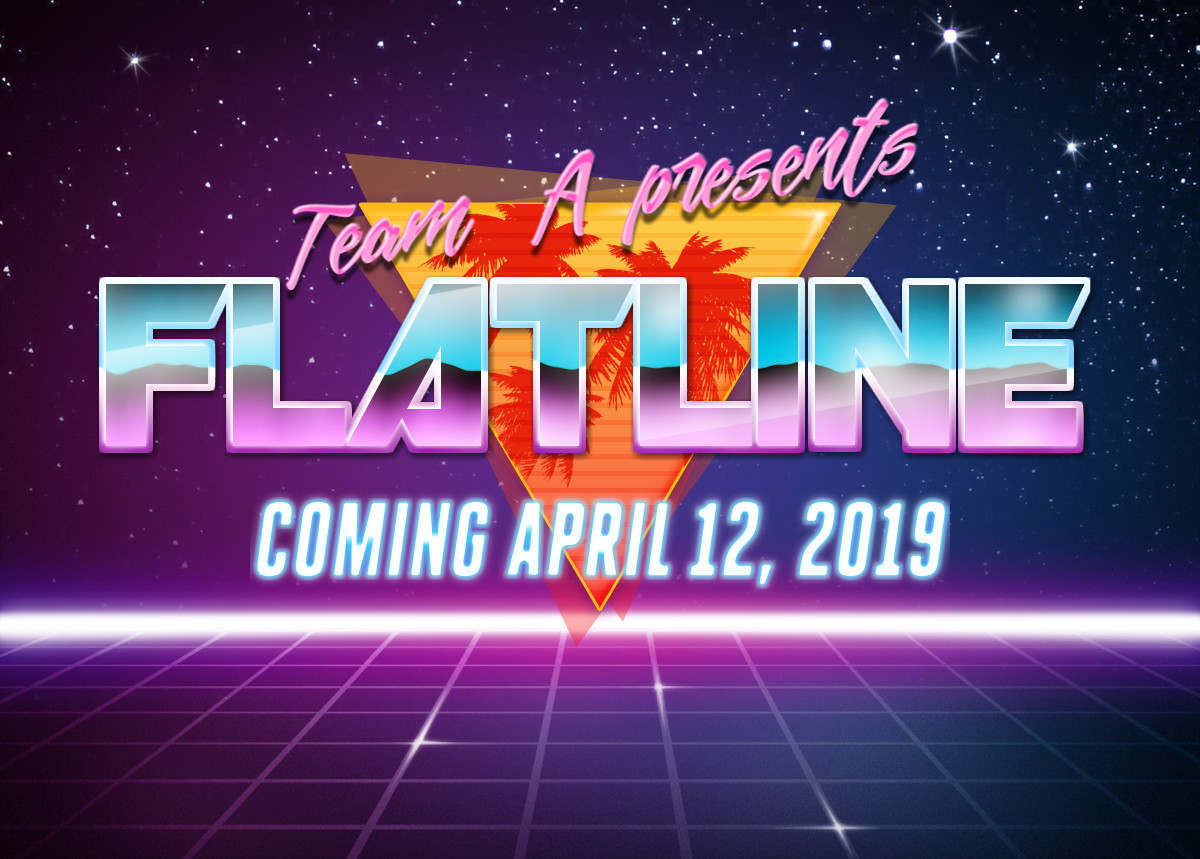
\includegraphics[width=1.0\linewidth]{title_art.jpg}
  % \caption{Title_art}
\label{fig:title_art}
\end{figure}

\name{} is a combat-based driving game aimed to test your skill to fight
against your enemies. Whether playing alone against AI or with friends, each
player find themselves driving a hovercraft in an arena pitted against each
other. Utilizing abilities, picking up power-ups, and the navigating the map,
everyone must destroy each other in a chaotic battle of strategy and wits
before the round is over.

The central constraint of the proposed features is development time available
to implement them. As a result, the following game features are subject to
change as development progresses.

\section{Gameplay}

\subsection{Terminology}

\textbf{Arena/Map:} The closed area where the game takes place.

\textbf{Ability:} The capabilities that a hovercraft can actively use.

\textbf{Bot:} An AI-controlled hovercraft. These hovercrafts are distinct from
player hovercrafts.

% TODO bot art here

\textbf{Player:} The individuals playing the game. May also interchangeably
refer to the hovercrafts controlled by the players for the sake of brevity,
especially in relation to the AI-controlled hovercrafts.

\begin{figure}[htpb]
  \centering
  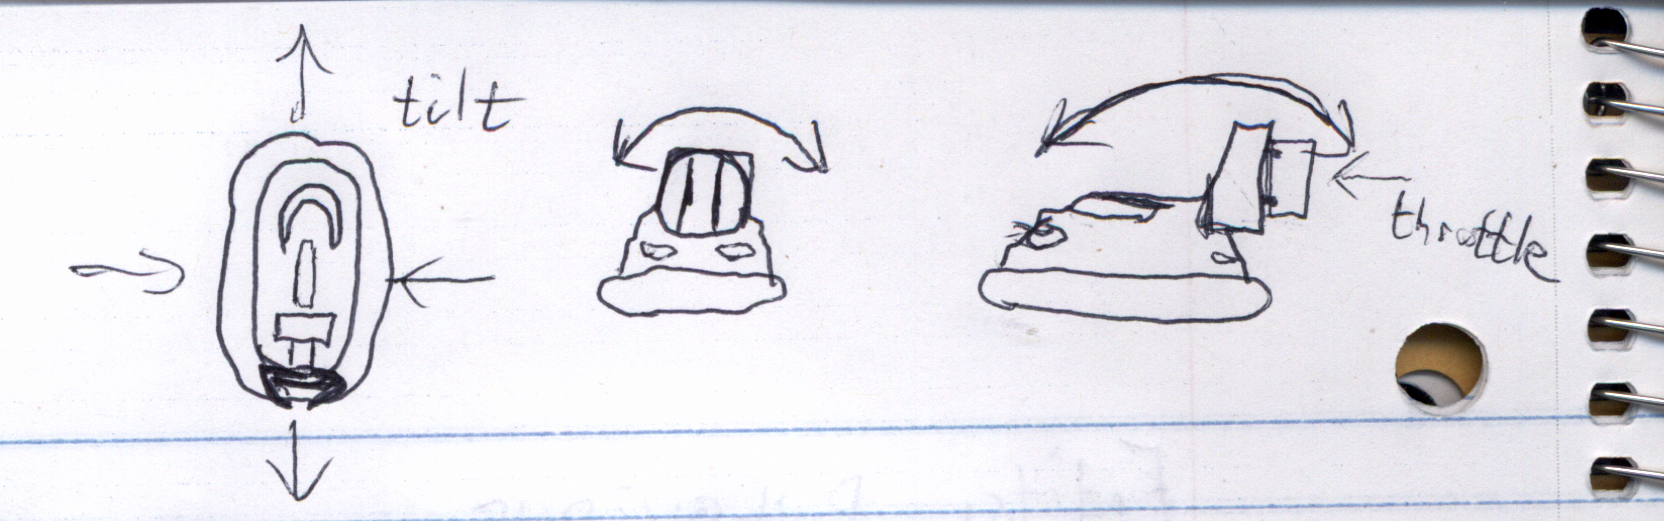
\includegraphics[width=0.8\linewidth]{Brainstorming_003.png}
  \caption{Sketch of the player hovercraft. The hovercraft should tilt based on
  its movement.}
\label{fig:Brainstorming_003}
\end{figure}

\textbf{Power-up:} An item located on the map that can be picked up by a player
by coming into contact with it. Upon pick-up, the player receives a temporary
effect, usually beneficial.

\subsection{Player Count}

The game supports single and local multiplayer, allowing for 1 to 4 players.
Local multiplayer would be split-screen multiplayer and would require multiple
input devices (XBOX controllers).

\subsection{Game Modes}

The main game mode proposed is \textbf{free-for-all}. At a low priority, other
modes may be developed if enough time is available.

\textbf{Free-for-all}

The game is composed of a single round that lasts for the duration of a timer.
Each player is placed in an arena to control a hovercraft with various
abilities. They must fight each other in a free-for-all battle with those
abilities, amidst a number of neutral bots roaming the arena to hunt down
players.

The central goal of the game is to gain the highest score possible before the
round is over. Players have the following means to gain score:
\begin{itemize}
  \item Damaging other player hovercrafts, which can only be done in
    multiplayer. This can be through the use of abilities accessible to every
    player.
  \item Destroying other player hovercrafts, which can only be done in
    multiplayer. If damage is done to a hovercraft's final hit point and it is
    destroyed, extra points are awarded.
  \item Destroying bots, which can be done in both single and multiplayer.
    Bot hovercrafts do not have all the abilities of player hovercrafts and
    so reward less points.
  \item Picking up power-ups. These help the player gain points by improving
    their abilities, but also innately give points when they are picked up.
\end{itemize}

\textbf{\textbf{King of the Hill}}

Similar to free-for-all, except a single player is designated the king. Only
the king is able to score points, meaning that players are incentivized to be
king for as long as possible to gain score. If another player destroys the
king, that player then switches to become the king.

\textbf{Co-op Survival}

Players must team up against a never-ending swarm of bots. Players only have
one life before they are out of the game. When all the players are destroyed,
the game ends.
\subsection{Arenas/Maps}

The game will feature a single map. Given the development time frame, a single
fun and polished map is preferable to multiple mediocre maps. It should be
``small'' to ``medium'' in size, to maintain a high player density to ensure
that players are always in the middle of the action, and do not get lost.

% TODO concept art of the map here

If time allows for additional maps, they may be added at a lower priority, but
the focus will still be on a singular main map. These additional maps should
provide a different purpose than the main map. For example, there could be
a small map designed for 1--2 players. This will lower the downtime as the
action with be closer and more compact.

\textbf{Environmental features}

\begin{itemize}
  \item Barriers/obstacles --- These can block movement and projectiles.
  \item Ramps --- Ramps lead to higher and lower platforms, or can be jumped
    off of over obstacles. This can provide better vision of certain parts of
    the map, give opportunities to jump between arenas.
  \item Pit --- Falling into the pit will instantly destroy the player
    hovercraft. Avoid at all costs or try to bump enemies into it.
  \item Speed pads --- Driving over these, will give a momentary boost of
    speed. Great for getting power-ups quicker, and chasing or escaping other
    players.
  \item Jump pads --- Driving over these, will give a vertical boost while
    maintaining horizontal momentum. Great for jumping over obstacles or
    reaching areas of higher elevation. % TODO is this okay?
\end{itemize}

\subsection{Players}

Players drive a hovercraft. They innately have full access to a number of
movement options and abilities from the start of the game.

\subsubsection{Health, Lives, and Damage}

Players start the game alive with a small set amount of hit points, which will
be explicitly displayed to the player. They can be damaged by the abilities of
other hovercrafts, lowering their current hit points. When all hit points is
removed, the player's hovercraft is destroyed.

When a player's hovercraft is destroyed, they lose some points and are
momentarily out of the game before respawning randomly at one of the respawn
points on the map. If another player destroyed said hovercraft, that player is
awarded points for the kill.

\subsubsection{Movement}

\begin{itemize}
  \item \textbf{Standard movement} --- A hovercraft does not rely on wheels to
    move and so can traverse in any lateral direction without needing to turn,
    meaning that strafing is possible.
  \item \textbf{Acceleration/braking} --- A hovercraft can accelerate an brake
    in any direction is it currently moving. It will often drift if a turn is
    made, even at relatively slow speeds, which can be both advantageous and
    disadvantageous. This is open to change as movement is play-tested to
    figure out what is fun and feels right.
  \item \textbf{Dashing} --- A hovercraft can dash in any direction. From
    a mobility standpoint, dashing can be used to catch up to other
    hovercrafts, reach power-ups faster, or lose others when being chased. From
    a defensive standpoint, it can be used to dodge attacks.
    % TODO should be blinking instead? Would make dashing through flame trail
    % more believable, as well as keeping momentum.
\end{itemize}

\subsubsection{Abilities}

Every hovercraft has 3 attack abilities that are available from the start of
the game.

\begin{itemize}
  \item \textbf{Rocket} --- A rocket launches forward straight out from the
    direction the hovercraft is facing until it hits a surface. Upon impact, it
    explodes, damaging everything in a radius around it. Being the only ranged
    attack, it is great for attacking distant enemies if aimed well, or when
    chasing other vehicles. The splash damage can be utilized with parts of the
    arena environment to hit enemies near walls easier, or to hit multiple
    enemies that are grouped together.
  \item \textbf{Spikes} --- Spikes temporarily extend in all directions from
    the hovercraft, damaging other vehicles that come in contact with it. Can
    be used both aggressively and defensively when other vehicles are nearby.
    It can also be used in combination with dashing to crash into enemies.
  \item \textbf{Flame trail} --- A trail of fire is created that follows the
    players path. Any hovercraft that contacts it is damaged. Great to use when
    being chased.
\end{itemize}

\subsection{Bots}

In all modes, a number of bots will be present on the map. With a visually
distinct design as players, bots will only target player hovercrafts. They are
weaker than players in that they have fewer hit points and fewer abilities, but
also award less points on kill. As a result, it is up to players to decide much
they want to focus on destroying bots versus other players in their strategy.

The capabilities of bots is open-ended as development progresses. Here is
a tentative priority list of bot functionality, from highest to lowest
priority.

\subsubsection{Movement}

% TODO discuss running away from players. This may result in bots clumping up
% and "running into walls" to move away from the player (such as the corners of
% the map).
It will be a requirement for bots to be able to target players to chase them.
They must be smart enough to recognize the presence of obstacles and general
map geometry to reach players in a reasonably direct path if possible.

At a lower priority, they may be given movement abilities or have more advance
movement decision-making such as:
\begin{enumerate}
  \item Speed boost. Bots will speed up towards players when a path is clear
    between the two. This will help them use their spikes to crash into the
    player for damage.
  \item Guard power-ups. Bots will recognize when power-ups are on the map and
    will guard the area to prevent the player from getting them.
\end{enumerate}

\subsubsection{Abilities}

To work with their basic chasing behaviour, the bots will, at minimum, be
equipped with the spikes ability, allowing them to ram into the player for
damage. Whether the spikes need to be activated or are always enabled will be
up to play-testing.

At a lower priority, they may given other abilities like the players:
\begin{enumerate}
  \item \textbf{Rockets} --- At its simplest, bots would be able to aim at
    players to fire rockets at them. More sophisticated, bots would be able to
    lead their shots based on the player's predicted trajectory and the rocket
    trajectory. Bot rockets may potentially travel slower than player rockets.
  \item \textbf{Flame trail} --- Bots will try to intercept the player's path
    to get them caught in the flame trail.
    % TODO discuss about dash/blink
\end{enumerate}

\subsubsection{Friendly fire}

Since the bots team up against the players, any damage they would deal to each
other would be purely accidental. At first glance, it would seem reasonable to
disable friendly fire so that bots would not destroy each other en masse.
However, friendly fire amongst bots may create in-game situations that would
add extra chaos, excitement or even humour to the game's atmosphere. If need
be, the bot count or respawn timing would be adjusted for balance to account
for these friendly kills.

Ultimately, the decision for allow for bot friendly fire will be up to
play-testing, and we will be open for it to work either way.

\subsection{Power-Ups}

Power-ups spawn at certain explicit power-up locations, where players can pick
them up by contacting them. Upon contact, the player that picked it up will
temporarily receive passive bonus for a set duration.

At minimum, we want there to be 3 power-up types. While there is no particular
priority in what power-ups to implement, we would ideally have one power-up for
each player ability. Here are some ideas:

\textbf{Rocket}
\begin{itemize}
  \item \textbf{Rapid-fire rockets} --- Rockets can be launched at a faster rate of
    fire. Good for spamming at a distance.
  \item \textbf{Homing rockets} --- Rockets will slightly home towards the
    closest target. Good for chasing.
  \item \textbf{Explosive rockets} --- Rockets will have a much larger impact
    radius. Good for taking out groups of enemies in small corridors.
\end{itemize}

\textbf{Spikes}
\begin{itemize}
  \item \textbf{Large spikes} --- Spike size increases, hitting enemies are
    further distances.
  \item \textbf{Passive spikes} --- Spikes are always enabled for the duration
    of the power-up.
  \item \textbf{Stunning spikes} --- Spikes will briefly disable enemy movement
    on contact. Can be used to set up another attack.
\end{itemize}

\textbf{Flame trail}
\begin{itemize}
  \item \textbf{Wide trail} --- The trail is much wider, easing the ability to
    catch opponents in their tracks.
  \item \textbf{Passive trail} --- The trail continuously lasts for the duration
    of the power-up.
  \item \textbf{Slowing trail} --- The trail slows the movement of enemies
    crossing it, making them vulnerable to attack.
  \item \textbf{Blocking trail} --- The trail cannot be bypassed, blocking
    enemies trying to cross it. Great for defense when being chased, or
    aggressively to trap enemies in an area.
\end{itemize}

\textbf{Other}
\begin{itemize}
  \item \textbf{Repair} --- The player gains an extra hit point.
  \item \textbf{Speed boost} --- The player gains a speed boost.
  \item \textbf{}\textbf{Shield} --- The player is invulnerable to abilities.
  \item \textbf{Invisibility} --- The player is invisible to other players and
    will not be targeted by bots.
\end{itemize}

\subsection{Difficulty}

\textbf{Single Player}

In a single player experience, the difficulty can arise
from a competitive approach in achieving a high-score. Whether one is
attempting to outperform their previous high scores, or compete with others'
high scores, players can improve their skills and learn new strategies to
improve. This self-imposed motivation to improve and compete can create new
levels of difficulty at a meta game level.

\textbf{Multiplayer}

Similar to single player, difficulty arises from the skills of opposing
players. As other players improve, so does oneself need to do to so to compete.
New strategies can arise in using abilities, power-ups, and parts of the map to
maximize points, as well as strategies to counter other players' play styles.

\subsection{Menu}

\section{Game Design}

\subsection{Aesthetic}

Visually, the game mainly follows a cyberpunk and TRON aesthetic. We are going
for a futuristic city at night appeal.

\begin{figure}[htpb]
  \centering
  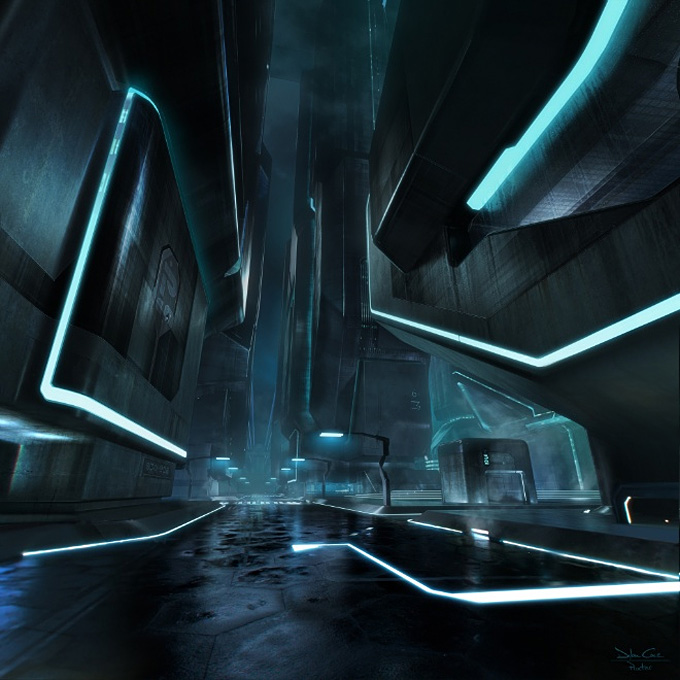
\includegraphics[width=0.8\linewidth]{theme01.jpg}
  \caption{Taking place at night, there will be a focus on artificial lights
  from buildings to illuminate the area.}
\label{fig:theme01}
\end{figure}

\begin{figure}[htpb]
  \centering
  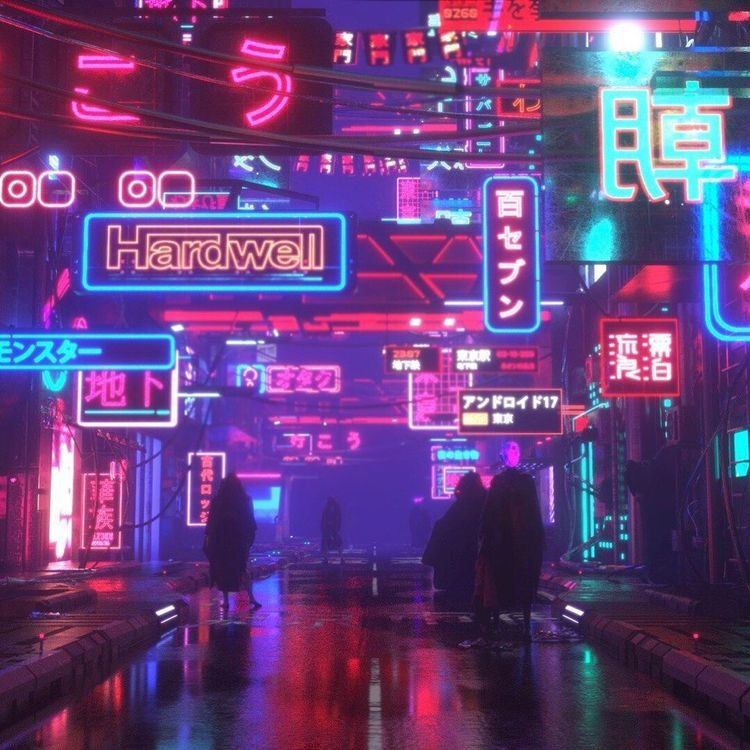
\includegraphics[width=0.8\linewidth]{theme02.jpg}
  \caption{Colourful neon lights will play an important role in creating
  a sense of warmth.}
\label{fig:theme02}
\end{figure}

\begin{figure}[htpb]
  \centering
  \includegraphics[width=0.8\linewidth]{theme03.jpg}
  \caption{There may be a contrast of lighter and darker arenas in the map,
  which may be used to highlight important areas such as power-up locations, or
ramps leading to different areas.}
\label{fig:theme03}
\end{figure}

\subsection{Inspiration}

\name{} is inspired from a number of other games:
\begin{itemize}
  \item \textbf{Akane} (2018) --- aesthetic
  \item \textbf{Crawl} (2017) --- king of the hill game mode
  \item \textbf{Mario Kart} (1992) --- free-for-all game mode and general combat design
  \item \textbf{Pac-Man} (1980) --- bot versus player design
  \item \textbf{ThinkTanks} (2003) --- Speed and jump pads
  \item \textbf{Tron} (1982) --- aesthetic and flame trail ability
\end{itemize}

\subsection{Designer Insight/Goals}

Here are some goals we have in mind for the project, as well as some insight
behind our design decisions from our team discussions.

\subsubsection{Vibe}

Playing \name{} should feel exciting and bring a sense of hype and energy,
similar to combat games like \textbf{Super Smash Bros} or \textbf{Street
Fighter}. This can be brought about through fast-paced gameplay, coupled with
action-packed sound effects and music.

\subsubsection{Role of AI}

The introduction of AI-controlled hovercrafts (bots) adds an interesting
element to the game, but also a few problems.

First, given our past experience and the time-frame creating the AI, we don't
believe the bots will be equally competent to a skilled human player. If bots
are given a hovercraft with equal capability to that of a player, it is
unlikely they will be able to utilize their abilities and movement sufficiently
to compete with players, or have sufficient game sense to outplay and counter
different play styles. This poses a problem for single-player, as competing
against a group of underperforming bots will not particularly fun or
challenging.

To address the challenge issue, it is possible to give bots point bonuses when
they score to improve their chances to beat players. However, this does not
necessarily address the fun issue, as the player will still experience fighting
against simple bots.

Instead, bots can be given an alternative role rather than replacing a player.
By explicitly giving them less capabilities than the player, and having them
exist in-game independent from the player count, they can add an extra depth to
the gameplay without heavily relying on the depth of their capabilities. The
benefit is that if the bots end up less capable than we initially planed, the
combat can still be just as fun since bots will be in greater numbers and team
up against the players. If they are more capable than we initially planned then
all the better, since this will simply make the gameplay more engaging.

\subsubsection{Driving System}

Since players are driving hovercrafts, the driving experience should model
that of a hovercraft. As a result, the driving model should feel somewhat
floaty, allowing for easier drifting. Without the constraint of wheels, the
players should be able to move in any lateral direction without needing to
turn, allowing for strafing.

However, if the hovercrafts are too floaty, they may be frustrating to control.
Driving needs to feel responsive, especially if sudden turns or braking are
done.

Our goal is for there to be a balance in the driving system for it to feel
somewhat floaty to imitate a hovercraft, and yet grounded enough to feel fun
and responsive. As we play-test the movement throughout the development, we
will iterate on this balance, and may even radically change how driving feels
if we believe it is best for the game.

\subsubsection{Learning Curve}

\textbf{Easy to Learn}

A core goal for game is for it to be easy to pick up and start playing.
Part of this involves controls that are intuitive to new players. While there
are a fair number of abilities, they are the same for everyone, meaning players
do not need to know the ins-and-outs of different vehicle abilities that they
themselves do not have access to.

Power-ups should feel intuitive to understand and use. They should not
introduce new mechanics or keybindings. It is frustrating for for new players
to ``waste'' power-ups in order to understand what they do, especially if they
are single-use. Instead, power-ups should augment already existing abilities
and clearly display in the UI which ability is improved.

\textbf{Hard to Master}

Players should be given opportunities to improve and apply their skill. Each
ability is distinct and requires its own skills to use.
% TODO

\subsubsection{Blue Shell Effect} % TODO balance?

\subsubsection{Combat}

% TODO
% health
% abilities no hit scan
% TODO move to insights
% All sources of damage deal a single point of damage. Hovercraft hit points are
% also a small, discrete value.
% This emphasizes dodging and avoiding abilities, and eases player
% understanding of how abilities work without needing to worry about different
% damage values.

\subsubsection{Performance}

\begin{itemize}
  \item \name{} should run at 60 fps for single player and 30 fps for
    multiplayer.
\end{itemize}


\subsection{Market Competition}

% TODO redo game competition
There are competitive elements to both the single-player and multiplayer
experience. In single-player, players can compete to achieve the highest score
possible, akin to competing to reach the top positions in the leader boards
in arcade games or certain online games. In other words, this can be be viewed
as a competitive asynchronous multiplayer experience.

In multiplayer, players can learn strategies to to counter 

\subsection{Game Genre} % Is this needed?

\name{} is a third-person combat-based driving game. It is designed to be
a fun party game that is easy for new players to pick up and play, while giving
the opportunity to those who want to master it the means to do so given.

It is developed for the PC, supporting Windows as a high priority and Mac and
Linux with lower priorities, using mouse and keyboard controllers. It will also
support XBOX 360 controller support, allowing for multiplayer modes.

\subsection{Branding}

\name{} is a new IP on its own.

\subsection{Target Market}

While violence is a core component of the gameplay, nothing is particularly
graphic due to the use of vehicles and the lack of blood and gore. We do not
intend there to be any mature themes in the game. We therefore believe that
\name{} is appropriately targeted for all ages 10 and above years of age.

\subsection{Gameplay Direction} % TODO needed?


\section{Concept Art}

\begin{figure}[htpb]
  \centering
  \includegraphics[width=0.8\linewidth]{Brainstorming_001.png}
  \caption{Rough sketches of the map, UI, and hovercraft}
\label{fig:Brainstorming_001}
\end{figure}

\begin{figure}[htpb]
  \centering
  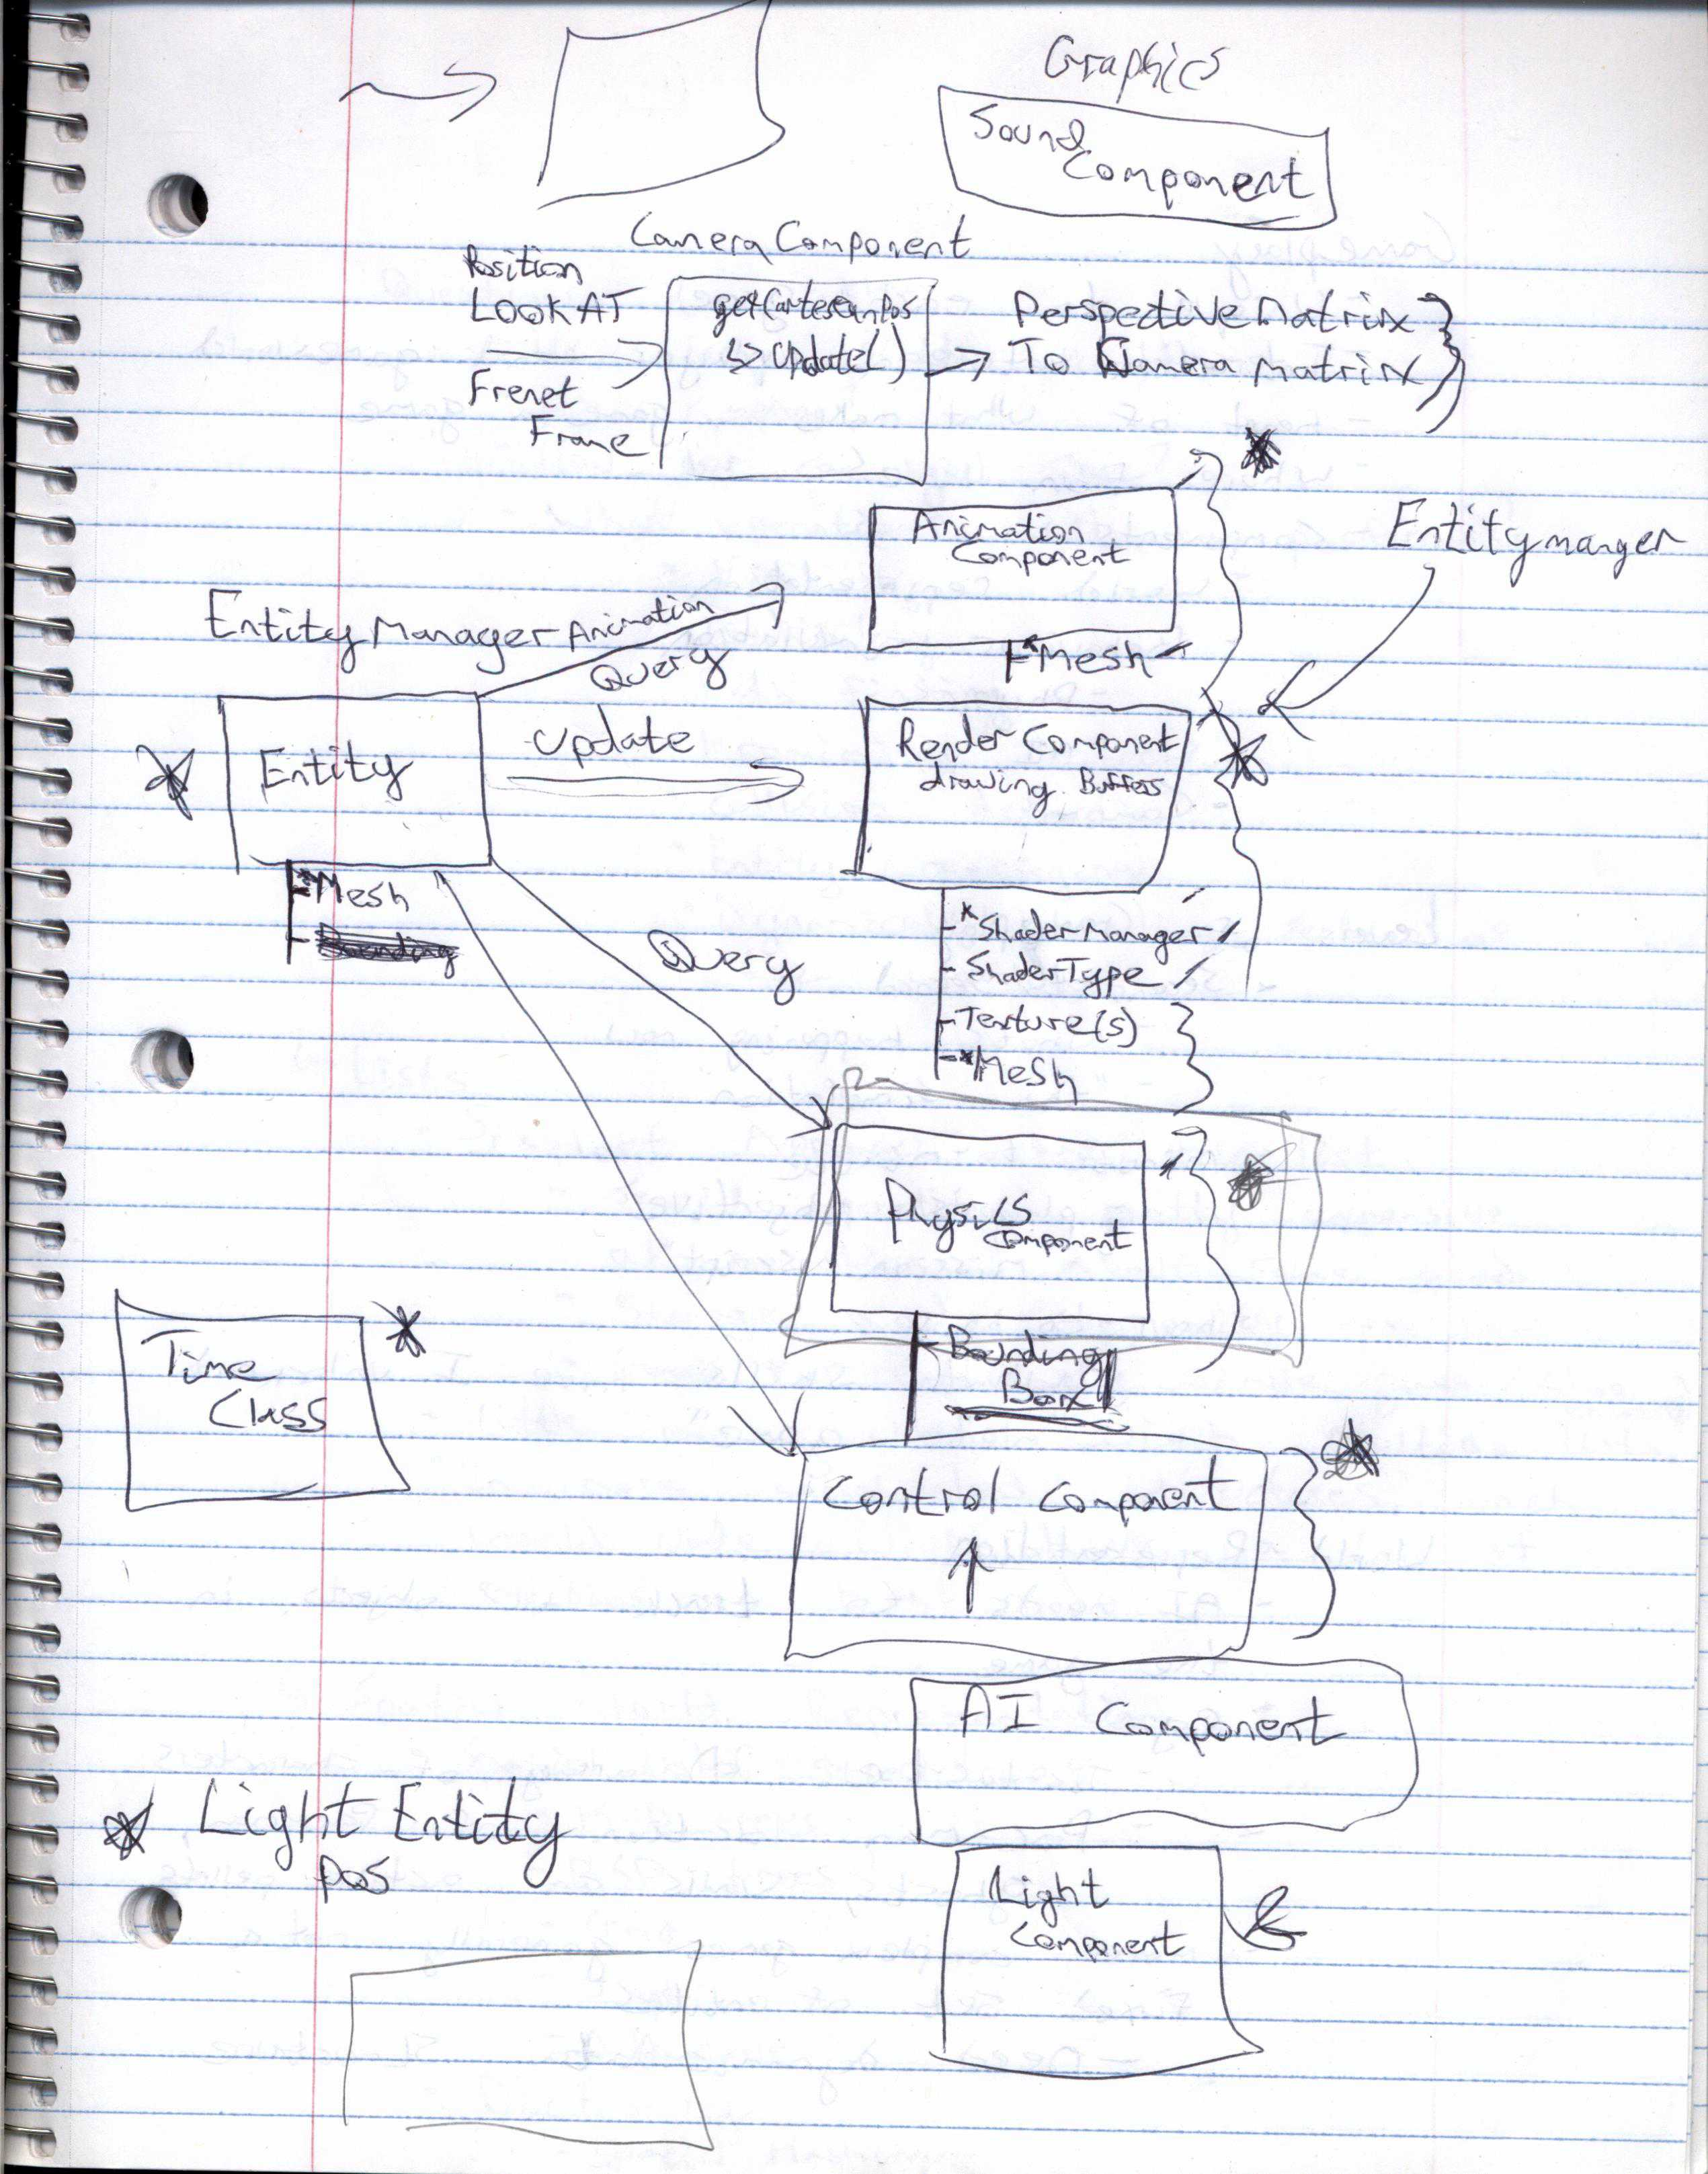
\includegraphics[width=0.8\linewidth]{Brainstorming_002.jpg}
  \caption{Early design of the game application framework}
\label{fig:Brainstorming_002}
\end{figure}

\end{document}
